\documentclass{article}
\usepackage{amsmath, amsthm, amssymb}
\usepackage{tikz}
\usepackage{array}

\begin{document}
\section*{\huge Mathematics Homework Sheet 1}
\begin{flushright}
   \textbf{Author: Abdullah Oguz Topcuoglu}
\end{flushright}

\section*{Problem 1}
Symmetry group S will consist of rotations and reflections.
\begin{itemize}
    \item Rotations: $R_{90}$, $R_{180}$, $R_{270}$
    \item Reflections: $T_x$, $T_y$, $T_d$, $T_{d'}$
    \item Identity: $I$
\end{itemize}

% draw a square and assign numbers to the corners
\begin{center}
   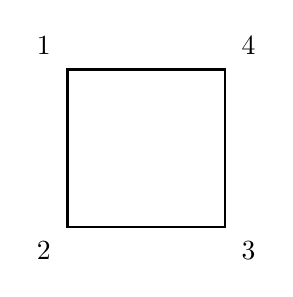
\begin{tikzpicture}
       \draw[thick] (0,0) rectangle (2,2);
       \node at (-0.3, -0.3) {2};
       \node at (2.3, -0.3) {3};
       \node at (-0.3, 2.3) {1};
       \node at (2.3, 2.3) {4};
   \end{tikzpicture}
\end{center}

$R_{i}$ rotates $i$ degrees clockwise. \\
$T_x$ reflects over the x-axis, $T_y$ reflects over the y-axis, $T_d$ reflects diagonally, and $T_{d'}$ reflects over the other diagonal.
\\
When we take a look at $S_4$, $S_4$ has 4! = 24 elements. \\
Our group S has 8 elements. \\
Lets start with identity $I$.
\begin{itemize}
   \item ()
\end{itemize}
Rotations:
\begin{itemize}
   \item $R_{90} = (1, 2, 3, 4)$
   \item $R_{180} = (1,3)(2,4)$
   \item $R_{270} = (1,4,3,2)$
\end{itemize}
Reflections:
\begin{itemize}
   \item $T_x = (1,2)(3,4)$
   \item $T_y = (1,4)(2,3)$
   \item $T_d = (1,3)$
   \item $T_{d'} = (2,4)$
\end{itemize}

So, when combined, \(S\) can be identified with this subset of \(S_4\):
\[
   \{ (), (1, 2, 3, 4), (1,3)(2,4), (1,4,3,2), (1,2)(3,4), (1,4)(2,3), (1,3), (2,4) \}
\]


\end{document}